\documentclass{article}
\usepackage{amsmath}
\usepackage{amsthm}
\usepackage{amsfonts}
\usepackage{amssymb}
\usepackage{bbold}
\usepackage{dsfont}
\usepackage{graphicx}
\usepackage{cleveref}
\usepackage{bm}
\usepackage{booktabs}
\usepackage{siunitx}
\usepackage{xcolor}
\usepackage[utf8]{inputenc}
\usepackage[english]{babel}
\newtheorem{definition}{Definition}
\newtheorem{example}{Example}
\newcommand{\exP}[1]{\mathrm{e}^{#1}}
\newcommand{\dif}{\mathrm{d}}
\renewcommand{\vec}[1]{\mathbf{#1}}
\newcommand{\pdagger}{{\phantom{\dagger}}}
\newcommand{\state}[1]{\vert #1\rangle}
\newcommand{\cstate}[1]{\langle #1\vert}
\newcommand{\tr}[1]{\mathrm{tr}\left\{#1\right\}}
\newcommand{\trs}[2]{\, \mathrm{tr}_{#1}\{#2\}}
\newcommand{\expc}[3]{\langle #1\vert #2 \vert #3\rangle}
\usepackage[doi=false,url=false,isbn=false,backend=bibtex,style=nature,natbib=true,sorting=none]{biblatex}
\bibliography{bib.bib}
\usepackage{geometry}
\geometry{
	a4paper,
	total={170mm,257mm},
	left=20mm,
	top=20mm,
}
\begin{document}
	
\title{Report 4: Corrected results and extension of analysis}
\author{Rudolf Smorka}
\maketitle
\tableofcontents
\section{Model}
The model considered for a chiral, single-stranded molecule, as proposed in Refs.~\cite{fransson2019chirality,fransson2020vibrational,Fransson_2021,fransson2021charge}, reads
\begin{align}
	\hat{H} &= \hat{H}_\mathrm{mol} + \hat{H}_\mathrm{env} + \hat{H}_\mathrm{sys-env}.
\end{align} 
The molecular Hamiltonian consists of electronic, vibrational and electron-vibrational contributions 
\begin{equation}
	\hat{H}_\mathrm{mol} = \hat{H}_\mathrm{el}  + \hat{H}_\mathrm{vib} + \hat{H}_\mathrm{el-vib}.
\end{equation}
The electronic contribution captures electron and spin transfer between different monomers of the molecule
\begin{equation}
	\begin{split}
		\hat{H}_\mathrm{el} &= \sum_{j,\sigma} \varepsilon_{j\sigma}^\pdagger \hat{d}_{j\sigma}^\dagger \hat{d}_{j\sigma}^\pdagger - t_0 \sum_{j\sigma} (\hat{d}_{j\sigma}^\dagger \hat{d}_{j+1,\sigma}^\pdagger + \mathrm{h.c.}) +\\& \lambda_0^\pdagger\sum_{j\sigma\sigma'} (i\hat{d}_{j\sigma}^\dagger (\vec{v}_j^{(+)}\cdot \bm{\sigma})_{\sigma\sigma'}^\pdagger \hat{d}_{j+2,\sigma'}^\pdagger + \mathrm{h.c.}).
	\end{split}
\end{equation}
An electron with spin $\sigma$ has energy $\varepsilon_{j\sigma}$ on site $j$, which is captured by the first term. An electron can hop between nearest-neighboring monomers with hopping amplitude $t_0$ (typically of the order $\SI{10}{\milli\electronvolt}-\SI{1}{\electronvolt}$). Further, electrons on next-nearest-neighboring sites are spin-orbit coupled (SOC) with amplitude $\lambda_0$ ($\lambda_0 \ll t_0$, with values of $\sim \SI{0.1}{\milli\electronvolt}-\SI{1}{\milli\electronvolt}$). This SOC-term is known as the  Kane-Mele model in the literature.
Further, the electrons couple to molecular (normal) vibrational modes, and the electron-vibrational Hamiltonian reads 
\begin{align}
	\hat{H}_\mathrm{el-ph} &= - t_1^\pdagger \sum_{j,\sigma}  \hat{d}_{j\sigma}^\dagger \hat{d}_{j+1\sigma}^\pdagger (\hat{a}_{j}^\dagger + \hat{a}_{j}^\pdagger) \\ & + \lambda_1^\pdagger\sum_{j,\sigma,\sigma'} (i \hat{d}_{j\sigma}^\dagger (\vec{v}_j^{(+)} \cdot \bm{\sigma})_{\sigma\sigma'}^\pdagger \hat{d}_{j+2\sigma'}^\pdagger +\mathrm{h.c.})(\hat{a}_{j}^\dagger + \hat{a}_{j}^\pdagger),\label{eq:HelPh}
\end{align}
The first term couples electron hopping between monomers to relative displacements of the monomers between which the hopping process happens, known as the Peierls-model. The second term is a contribution to this monomer displacement due to SOC. Finally, the vibrational energy reads 
\begin{equation}
	\hat{H}_\mathrm{ph} = \sum_{j} \omega_{j}^\pdagger \hat{a}_{j}^\dagger \hat{a}_{j}^\pdagger.
	\label{eq:HPh} 
\end{equation}
This molecule is coupled to two leads of spin-full, noninteracting electrons
\begin{equation}
	H_\mathrm{env} = \sum_{\ell k\sigma} \varepsilon_{\ell k\sigma}^\pdagger c_{\ell k\sigma}^\dagger c_{\ell k\sigma}^\pdagger \label{eq:LeadHamiltonian}
\end{equation}
and the system-environment coupling is linear in the electronic operators of the molecule and lead
\begin{align}
	H_\mathrm{sys-env} &= \sum_{\sigma\sigma'}(\nu_{L\sigma\sigma'}^\pdagger c_{N_L\sigma}^\dagger d_{1\sigma'}^\pdagger + \nu_{R\sigma\sigma'}^\pdagger c_{1_R\sigma}^\dagger d_{\mathbb{M}\sigma'}^\pdagger + \mathrm{h.c.}). \label{eq:LeadSysHamiltonian}
\end{align} 
Note, that only at the first and last site of the molecule are coupled to the respective leads. Observables of interest are the local electronic populations
\begin{equation}
	n_{i\sigma}(t) = \tr{\rho_S(t) \hat{n}_{i\sigma}},
\end{equation}
with the reduced density matrix $\rho_S(t) = \mathrm{tr}_\mathrm{env}\{\rho(t)\}$, from which one obtains the local spin polarization $s^z_i = n_{i\uparrow}-n_{i\downarrow}$. Charge currents from lead $\ell$ to the system are defined as
\begin{equation}
	I_\ell(t) = \tr{\rho(t) \frac{\dif}{\dif t}\sum_k c^\dagger_{k\ell}c^\pdagger_{k\ell}}.
\end{equation}
Within the MF-HEOM, charge currents are obtained from the trace of the current matrices 
\begin{equation}
	I_\ell(t) = \tr{\Pi_\ell(t)}
\end{equation}
while within the TT-HEOM, charge currents are obtained by \cite{ke2022hierarchical}
\begin{equation}
	\begin{split}
		I_\ell(t) = &\sum_{i\ell} \frac{\Gamma_{i\ell}}{2}(\delta_{\ell, L}- \delta_{\ell, R}) \expc{\mathbb{I}_0}{\hat{d}_i^-\hat{d}_i^+ - \hat{d}_i^+\hat{d}_i^- }{\Psi(t)} \\ + i & \sum_{k=1}^K (-1)^{\sigma_k }\sqrt{\Gamma_{i_k\ell_k}}(\delta_{\ell_k,L}- \delta_{\ell_k,R})\expc{\mathbb{I}_{\bm{1}_k}}{\hat{d}_{i_k}^{\sigma_k}}{\Psi(t)}.
	\end{split}
\end{equation}
Further, we investigate local currents between sites $j,k$ of the molecule, defined as
\begin{equation}
	I_{jk}(t) =\frac{i}{2} \tr{H_{jk}(t)\rho_{kj}(t)-\rho_{jk}(t)H_{kj}(t)}.
\end{equation}
\section{Born-Oppenheimer potential energy of the three-site Fransson model}
The Born-Oppenheimer approximation yields the following Hamiltonian for the three-site Fransson model
\begin{equation}
	H_\mathrm{BO} = \begin{pmatrix}
		\left(\varepsilon_1 + \frac{\omega_0^2 X_1^2}{2}\right) \mathds{1} & -(t_0 +t_1\sqrt{2\omega_0}X_1)\mathds{1} & (\lambda_0 + \lambda_1\sqrt{2\omega_0}X_1)\vec{v}_{13}^{(+)}\cdot\bm{\sigma}\\
		-(t_0 +t_1\sqrt{2\omega_0}X_1)\mathds{1} & \left(\varepsilon_2 + \frac{\omega_0^2 X_2^2}{2}\right) \mathds{1} & -(t_0 +t_1\sqrt{2\omega_0}X_2)\mathds{1} \\
		(\lambda_0 + \lambda_1\sqrt{2\omega_0}X_2)\vec{v}_{31}^{(+)}\cdot\bm{\sigma}&  -(t_0 +t_1\sqrt{2\omega_0}X_2)\mathds{1} & \varepsilon_3 \mathds{1}
	\end{pmatrix}.\label{eq:BO_Hamiltonian_Fransson_1x3}
\end{equation}
The adiabatic potential energy surfaces for various values of $t_1$ and $\lambda_1$ (other parameters are the same as in \cref{sec:1_Comp_TTHEOM_MFHEOM}) are shown in \cref{fig:PES_1x3_lambda1_t1_Var}. Note that the Hamiltonian \cref{eq:BO_Hamiltonian_Fransson_1x3} is 6-dimensional due to the spin of the electron. However, because the spin-orbit coupling $\lambda_0$ is 40 times smaller than $t_0$ and 4 times smaller than $t_1$, the two-fold degeneracy of eigenstates is lifted on an energy-scale much smaller than variations of the energies when varying vibrational displacements. Shown are the influence of $t_1$ alone (a$_1$)-(a$_3$), $\lambda_1$ alone (b$_1$)-(b$_3$), and the case where $t_1=\lambda_1$ (c$_1$)-(c$_3$). Since $\lambda_1=\frac{t_1}{40}$, the BO-potential energy surfaces of the Fransson model investigated in the previous section are very similar to the ones shown in \cref{fig:PES_1x3_lambda1_t1_Var} (a$_1$)-(a$_3$). We denote the states of the purple PES by $S_1,S_2$, the green one by $S_3,S_4$ and the gold one by $S_5,S_6$.
Notable points are the avoided crossings of states $S_1,S_2$ with $S_3,S_4$ at $X_1=-69,-160$ and states $S_3,S_4$ with $S_5,S_6$ at $X_1=-159,-160$. 
\begin{figure}[!h]
	\centering
	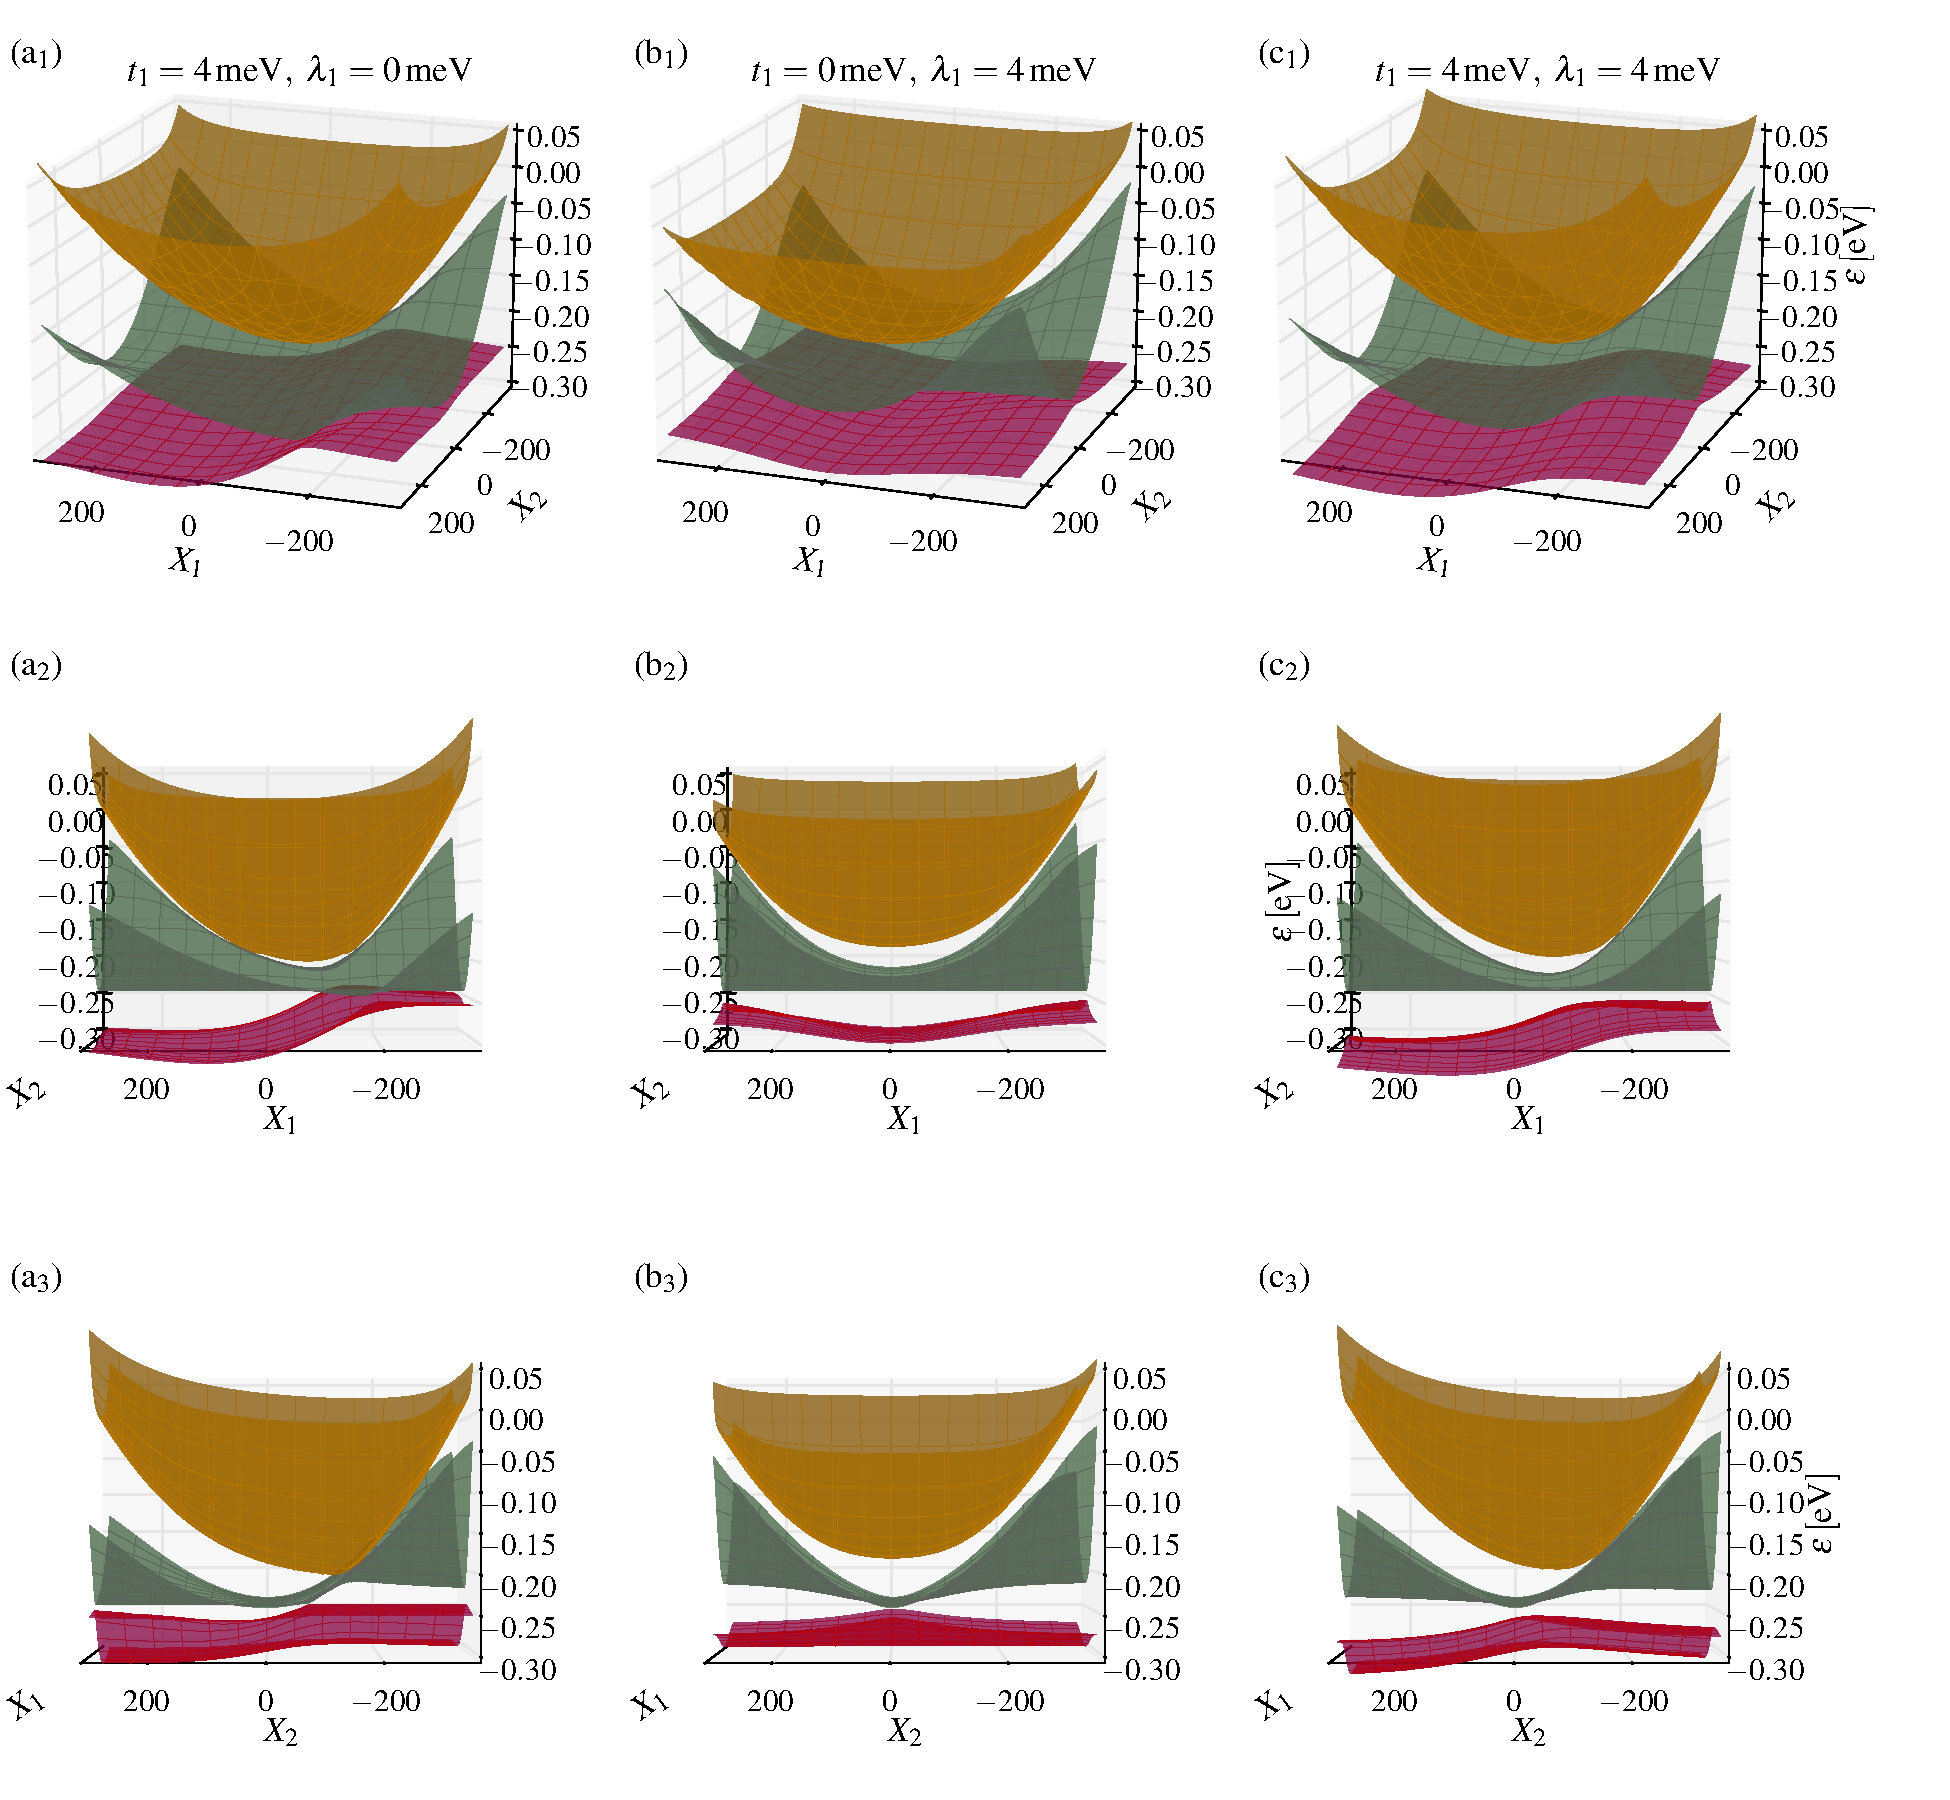
\includegraphics[width=0.99\textwidth]{figs/PES_1x3_SOC0.001_tPh0.004_SOCPh0.0001_multiState_multiAngle.pdf}
	\caption{Adiabatic potential energy surfaces for the Fransson model with molecular size $\mathbb{M}=1\times 3$, $t_0=\SI{40}{\milli\electronvolt}$, $\lambda_0 = \SI{0.1}{\milli\electronvolt}$ and $\omega_0 = \SI{2}{\milli\electronvolt}$ for $t_1=\SI{4}{\milli\electronvolt}$ and $\lambda_1 = \SI{0}{\milli\electronvolt}$ (a$_1$)-(a$_3$), $t_1=\SI{0}{\milli\electronvolt}$ and $\lambda_1 = \SI{4}{\milli\electronvolt}$ (b$_1$)-(b$_3$), and $t_1=\SI{4}{\milli\electronvolt}$ and $\lambda_1 = \SI{4}{\milli\electronvolt}$ (c$_1$)-(c$_3$)}\label{fig:PES_1x3_lambda1_t1_Var}
\end{figure}
\begin{figure}[!h]
	\centering
	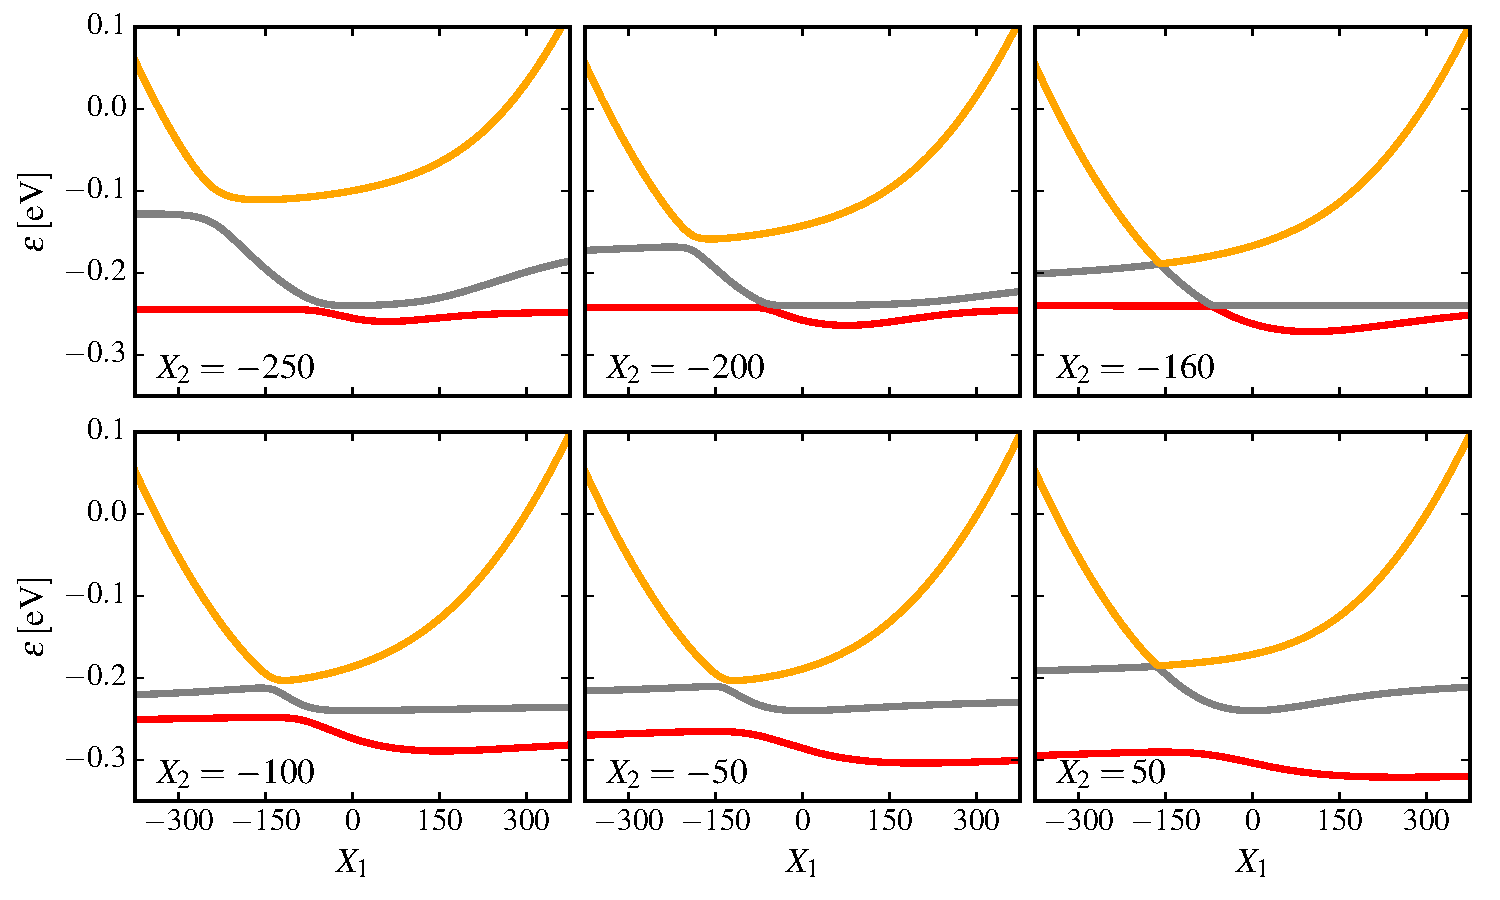
\includegraphics[width=0.99\textwidth]{figs/PES_1x3_SOC0.001_tPh0.004_SOCPh0.0001_multiState_cuts.pdf}
	\caption{BO-states for fixed $X_2$ and varying $X_1$. Parameters are as above.}
\end{figure}
\begin{figure}[!h]
	\centering
	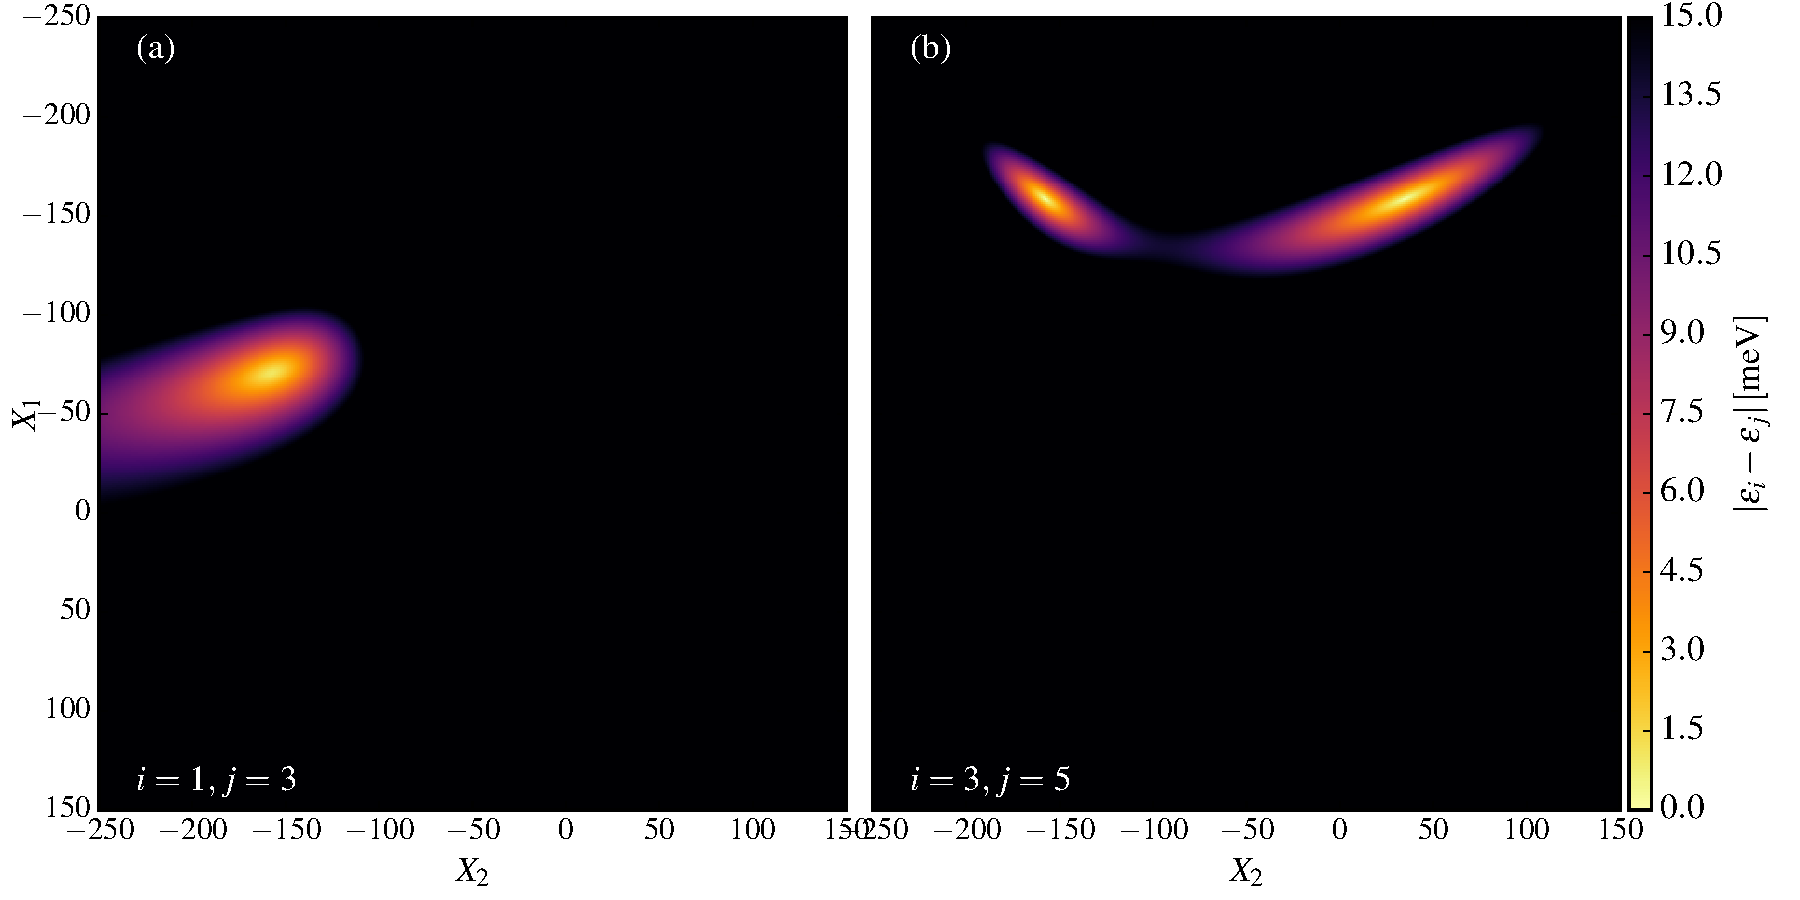
\includegraphics[width=0.99\textwidth]{figs/PES_1x3_SOC0.001_tPh0.004_SOCPh0.0001_multiState_difference.pdf}
	\caption{Absolute difference between BO-eigenstates $S_1$ and $S_3$ (a) and $S_3$ and $S_5$ (b) in the vibrational displacement space.} 
\end{figure}
\clearpage
\section{Comparison of TT-HEOM with MF-HEOM}\label{sec:1_Comp_TTHEOM_MFHEOM}
\subsection{Fransson model}
Parameters: $\mathbb{M}=1\times 3$, $t_0 = \SI{40}{\milli\electronvolt}$, $\lambda_0 = \SI{1}{\milli\electronvolt}$, $t_1=\SI{4}{\milli\electronvolt}$, $\lambda_1 = \SI{0.1}{\milli\electronvolt}$, $\Gamma_0 = \SI{4}{\milli\electronvolt}$ (with lead spin polarization $P = 0.5$), $V=\SI{0.48}{\volt}$ and $T =\SI{ 300}{K}$.
The following vibrational frequencies are investigated: $\omega_0 = \SI{2}{\milli\electronvolt}$ and $\omega_0=\SI{120}{\milli\electronvolt}$.  

We start with the case low vibrational frequency first, shown in \cref{fig:TTHEOM_MFHEOM_comp_w0_0.05}. There we plot the symmetrized current (a) and the spin-down population on the first site (b), comparing the MF-HEOM results (weighted average over $n=9000$ trajectories sampled from the thermal Wigner distribution for a harmonic oscillator) with TT-HEOM results (various ranks $r$ and number of vibrational states $n_\mathrm{vib}$ for each vibrational mode). Even a rank of $r=200$ and $n_\mathrm{vib}=30$ vibrational states are not sufficient for converging the TT-HEOM results. Although the symmetrized current seems to be converged with increasing the rank and the number of vibrational states in the time-interval until $\sim\SI{5}{\femto\second}$, the population rises above one for all investigated ranks. The unphysical population is obtained already in the first time-step of the calculation.
\begin{figure}
	\centering
	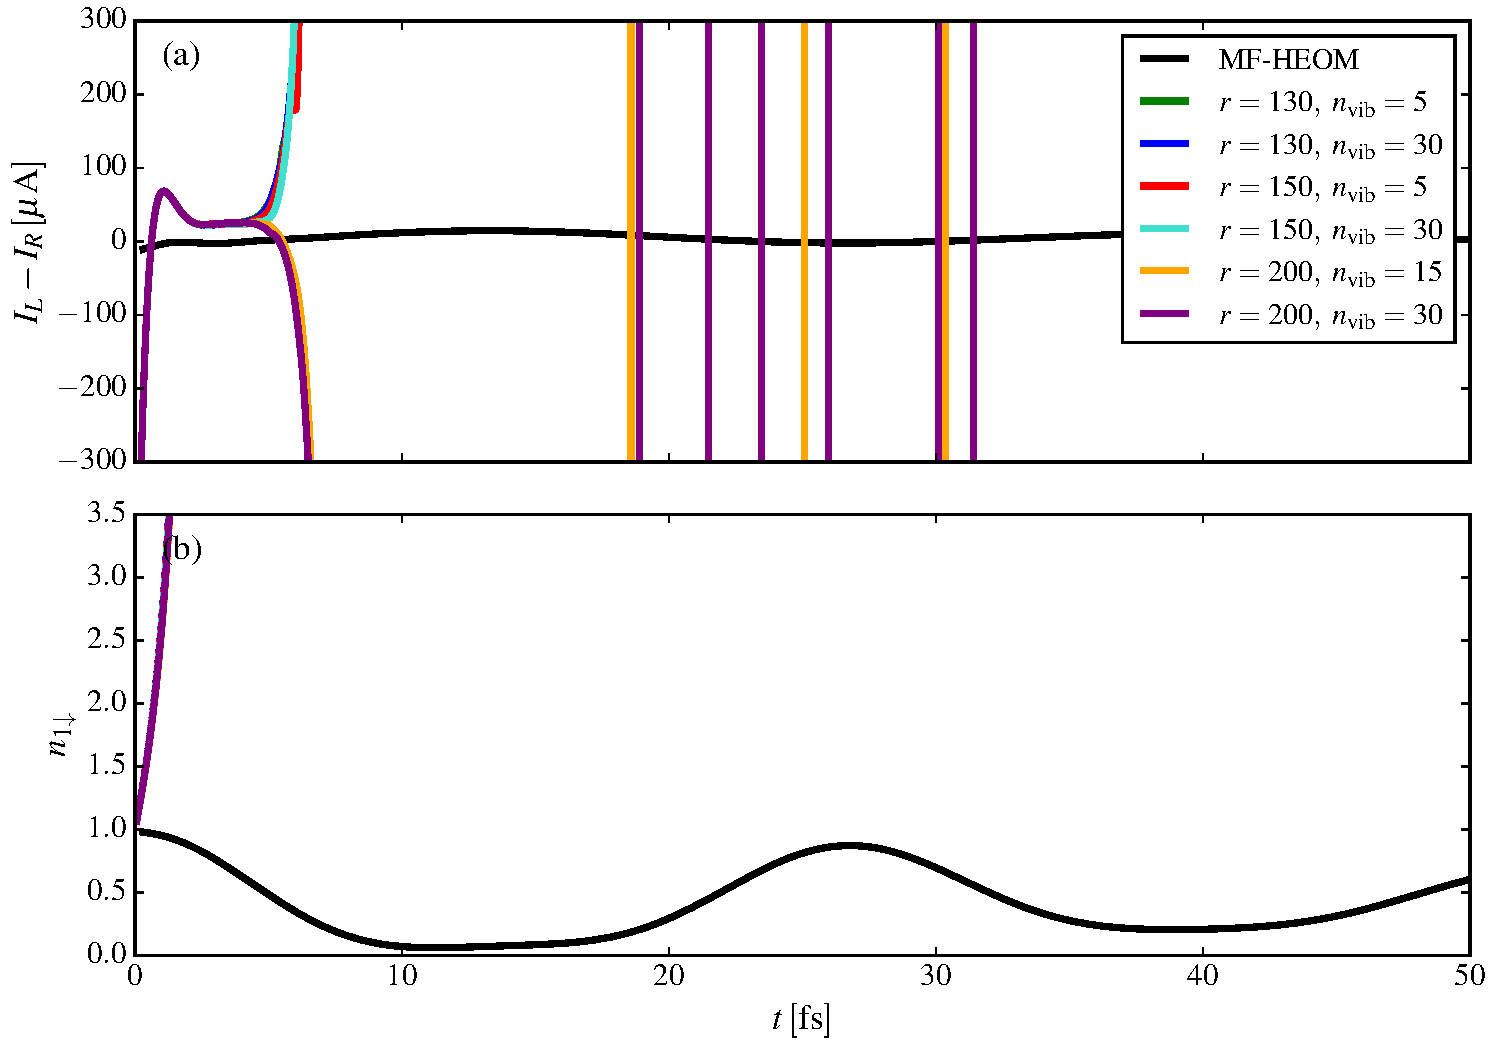
\includegraphics[width=0.9\textwidth]{figs/Comparison_TTHEOM_MFHEOM_1x3_w0_0.05_Gamma0.1t0.pdf}
	\caption{Comparison of MF-HEOM (sample size $n=9000$) with TT-HEOM (for various rank $r$ and number of vibrational states $n_\mathrm{vib}$): Symmetrized current (a) and population of spin-down electron on the first site (b) for $\omega_0 = \SI{2}{\milli\electronvolt}$. }\label{fig:TTHEOM_MFHEOM_comp_w0_0.05}
\end{figure}

We now turn to the case with higher vibrational frequency $\omega_0=\SI{120}{\milli\electronvolt}$, shown in \cref{fig:TTHEOM_MFHEOM_comp_w0_3}. In essence, the time-scale on which the symmetrized current and the population diverges within the TT-HEOM, does not significantly change upon increasing the vibrational frequency.
\begin{figure}
	\centering
	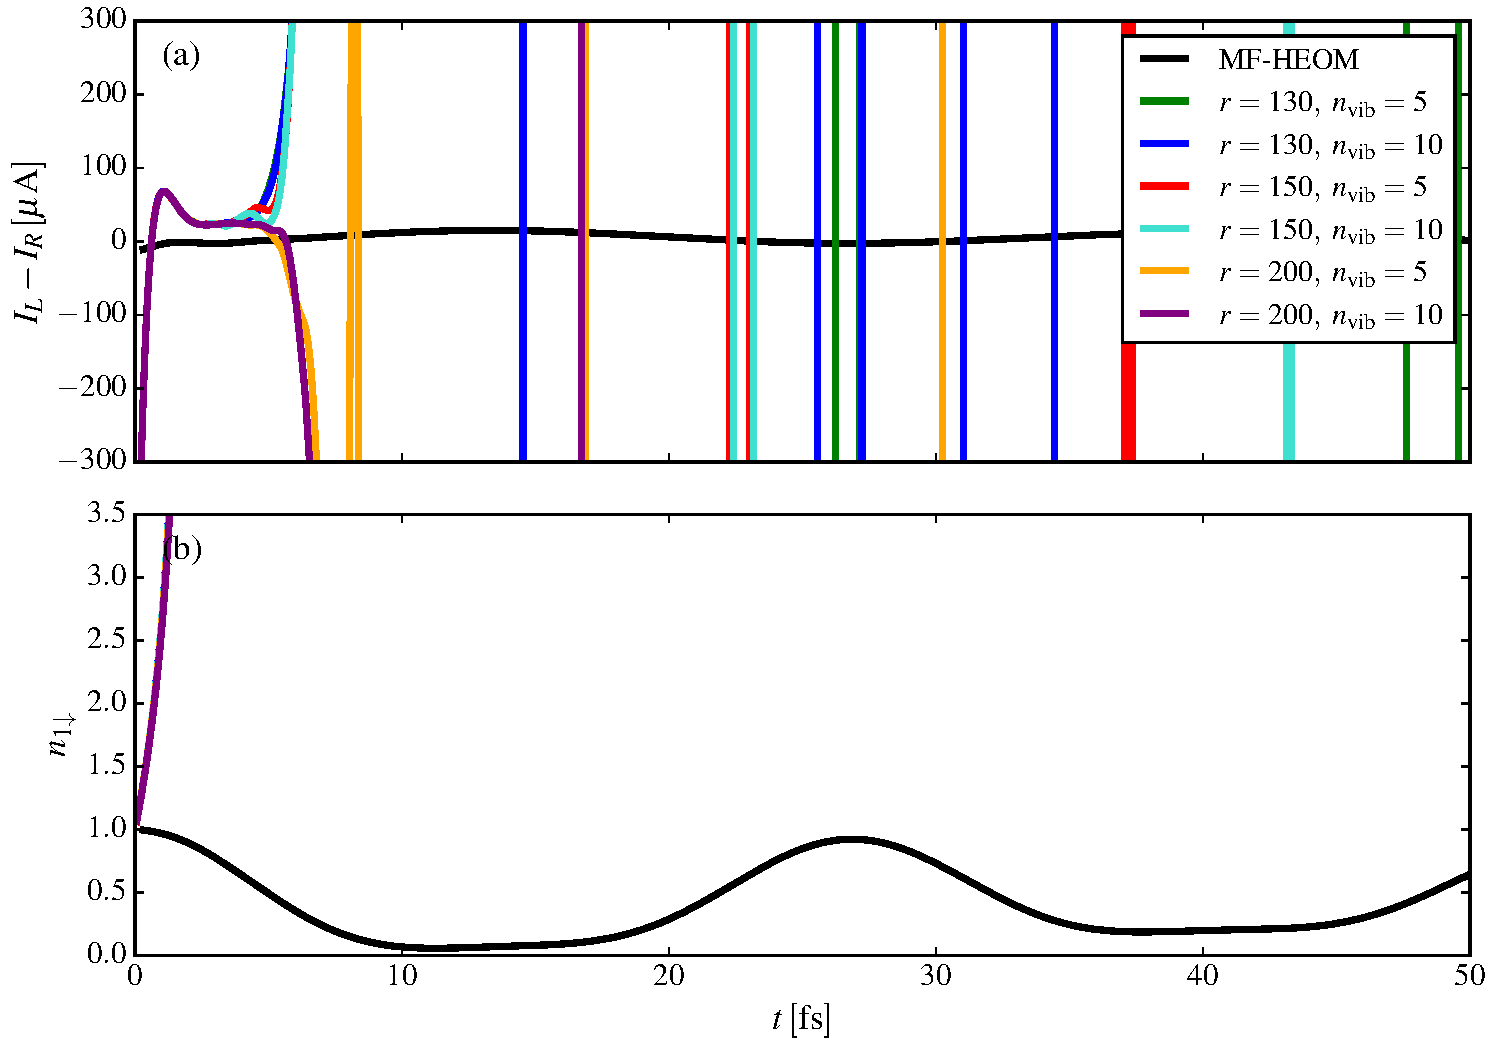
\includegraphics[width=0.9\textwidth]{figs/Comparison_TTHEOM_MFHEOM_1x3_w0_3.0_Gamma0.1t0.pdf}
	\caption{Same as \cref{fig:TTHEOM_MFHEOM_comp_w0_0.05} for $\omega_0 = \SI{3}{\milli\electronvolt}$. }\label{fig:TTHEOM_MFHEOM_comp_w0_3}
\end{figure}
\subsection{Single-site: Holstein model}
\subsection{Two sites: Peierls model}




\printbibliography
\end{document}




